\documentclass[12pt, a4paper]{article}

\usepackage[utf8]{inputenc}
\usepackage[spanish]{babel}
\usepackage{titling}
\usepackage[left=2cm,right=2cm,top=2cm,bottom=2cm]{geometry}
\usepackage{enumerate}
\usepackage{amsmath}
\usepackage{graphicx}
\usepackage{caption}

\usepackage{listings}%-para agregar codigo-
\usepackage[usenames,dvipsnames]{color}
\usepackage{color}%------------------------

%---------------------importar codigo desde archivos cpp----------------------------
\lstloadlanguages{C++}
\lstnewenvironment{code}
	{%\lstset{	numbers=none, frame=lines, basicstyle=\small\ttfamily, }%
	 \csname lst@SetFirstLabel\endcsname}
	{\csname lst@SaveFirstLabel\endcsname}
\lstset{% general command to set parameter(s)
	language=C++, basicstyle=\small\ttfamily, keywordstyle=\slshape,
	emph=[1]{tipo,usa}, emphstyle={[1]\sffamily\bfseries},
	morekeywords={tint,forn,forsn},
	basewidth={0.47em,0.40em},
	columns=fixed, fontadjust, resetmargins, xrightmargin=5pt, xleftmargin=15pt,
	flexiblecolumns=false, tabsize=2, breaklines,	breakatwhitespace=false, extendedchars=true,
	numbers=left, numberstyle=\tiny, stepnumber=1, numbersep=9pt,
	frame=l, framesep=3pt,
    basicstyle=\ttfamily,
    keywordstyle=\color{blue}\ttfamily,
    stringstyle=\color{magenta}\ttfamily,
    commentstyle=\color{RedOrange}\ttfamily,
    morecomment=[l][\color{OliveGreen}]{\#}
}

\lstdefinestyle{C++}{
	language=C++, basicstyle=\small\ttfamily, keywordstyle=\slshape,
	emph=[1]{tipo,usa,tipo2}, emphstyle={[1]\sffamily\bfseries},
	morekeywords={tint,forn,forsn},
	basewidth={0.47em,0.40em},
	columns=fixed, fontadjust, resetmargins, xrightmargin=5pt, xleftmargin=15pt,
	flexiblecolumns=false, tabsize=2, breaklines,	breakatwhitespace=false, extendedchars=true,
	numbers=left, numberstyle=\tiny, stepnumber=1, numbersep=9pt,
	frame=l, framesep=3pt,
    basicstyle=\ttfamily,
    keywordstyle=\color{blue}\ttfamily,
    stringstyle=\color{magenta}\ttfamily,
    commentstyle=\color{RedOrange}\ttfamily,
    morecomment=[l][\color{OliveGreen}]{\#}
}

\def\nbtitle#1{\begin{Large}\begin{center}\textbf{#1}\end{center}\end{Large}}
\def\nbsection#1{\section{#1}}
\def\nbsubsection#1{\subsection{#1}}
\def\nbcoment#1{\begin{small}\textbf{#1}\end{small}}
\newcommand{\comb}[2]{\left( \begin{array}{c} #1 \\ #2 \end{array}\right)}
\def\complexity#1{\texorpdfstring{$\mathcal{O}(#1)$}{O(#1)}}
 \newcommand\cppfile[2][]{
\lstinputlisting[style=C++,linerange={#1}]{#2}
}
%------------------------------------------------------------------------------

\newcommand{\subtitulo}[1]{\begin{center}\textbf{#1}\end{center}}

\title{\textbf{Estructuras de datos}}
\author{Wilmer Emiro Castrillón Calderón}

% Para que busque los archivos en una carpeta arriba
\graphicspath{{../}}
\newcommand*\lstinputpath[1]{\lstset{inputpath=#1}}
\lstinputpath{../}
%------------------------------------------------------------------------------

\begin{document}
	\maketitle
	
	%<*Capitulo>
	
	\section{Tablas aditivas}
	Son estructuras de datos utilizadas para realizar operaciones acumuladas sobre un conjunto de datos estáticos 
	en un rango específico, es decir, ejecutar una misma operación(como por ejemplo la suma) sobre un intervalo 
	de datos, se asume que los datos en la estructura no van a cambiar. Estas estructuras también son conocidas como 
	\textit{Summed-area table} para el procesamiento de imágenes, a pesar de su nombre no necesariamente son 
	exclusivas para operaciones de suma, pues la idea general es aplicable a otras operaciones.
	
	Durante el cálculo de una misma operación sobre diferentes rangos se presenta superposición de problemas, las 
	tablas aditivas son utilizadas para reducir la complejidad computacional aprovechando estas superposiciones
	utilizando programación dinámica.
	
	\subtitulo{Ejemplo inicial.}
	
	Dado un vector V = \{5,2,8,2,4,3,1\} encontrar para múltiples consultas la suma de todos los elementos en un rango
	[i,j], indexando desde 1, por ejemplo con el rango [1, 3] la suma es [5+2+8] = 15.
	
	La solución trivial es hacer un ciclo recorriendo el vector entre el intervalo [i,j], en el peor de los casos se
	debe recorrer todo el vector, esto tiene una complejidad $O(n)$ puede que para una consulta sea aceptable, pero
	en casos grandes como por ejemplo un vector de tamaño $10^{5}$ y una cantidad igualmente grande de consultas el
	tiempo de ejecución se hace muy alto, por lo tanto se hace necesario encontrar una mejor solución.	
	
	La operación suma tiene propiedades que nos pueden ayudar a resolver este problema de una forma mas eficiente:
	\begin{enumerate}[1.]
		\item La suma es asociativa es decir, se cumple: $a+(b+c)=(a+b)+c$, esto indica que sin importar 
			la agrupación que se realice el resultado sera igual (no confundir con propiedad conmutativa).
		\item La suma posee elemento neutro, es decir existe un $\beta$ tal que $a + \beta = a$, en la suma 
			$\beta = 0$.
		\item La suma tiene operación inversa, es decir existe una operación que puede revertir la suma, la cual 
			es la resta: si $a+b=c$ entonces $c-a=b$.
	\end{enumerate}
	
	Considerando las anteriores propiedades el problema se puede trabajar desde otro enfoque, primero se puede
	definir $suma(x)$ = $\sum_{k=1}^{x} V_{k}$, ahora tomando como ejemplo una consulta en el rango [3,5] 
	del vector $V$, se tomara convenientemente: $suma(2) = V_{1}+V_{2}$ y $suma(5) = V_{1}+V_{2}+V_{3}+V_{4}+V_{5}$,
	pero se necesita encontrar $V_{3}+V_{4}+V_{5}$, usando la propiedad asociativa se obtiene: 
	$(V_{1}+V_{2})+(V_{3}+V_{4}+V_{5})=(V_{1}+V_{2}+V_{3}+V_{4}+V_{5})$ y usando la propiedad inversa se llega a:
	$(V_{3}+V_{4}+V_{5})=(V_{1}+V_{2}+V_{3}+V_{4}+V_{5})-(V_{1}+V_{2})$ por lo tanto 
	$(V_{3}+V_{4}+V_{5})=suma(5)-suma(2)$. De esta manera el problema se puede generalizar como 
	$\sum_{k=i}^{j} V_{k} = suma(j) - suma(i-1)$ cuando $i \neq 1$ y $suma(j)$ cuando $i=1$.
	
	Ahora pre-calculando $suma(x)$ se puede dar una solución inmediata a cada consulta, esto se puede resolver 
	utilizando un enfoque básico de programación dinámica. Para encontrar $suma(x)$ se puede reescribir como: 
	$suma(x) = V_{x} + suma(x-1)$ con caso base $suma(1)=V_{1}$ y por definición la operación acumulada sobre un 
	conjunto vacío es igual al elemento neutro, a partir de esto se puede obtener la siguiente solución en 
	C++ con consultas indexando desde 1.
	\cppfile[6-14]{Estructuras_de_datos/codigos/tablas_aditivas.cpp}
	
	De manera general las tablas aditivas son aplicables a cualquier operación que posea las tres propiedades 
	descritas anteriormente: ser asociativa, tener elemento neutro y operación inversa, por ejemplo la suma,
	multiplicación o el operador de bits XOR.

	\subtitulo{Tablas aditivas en 2D}
	
	Las operaciones acumuladas no solo se pueden usar sobre una dimension, sino también sobre n-dimensiones, en estos
	casos se debe trabajar con el principio de inclusión-exclusión pues se debe considerar mejor las operaciones entre
	intervalos, si no tiene en cuenta este principio las soluciones contendrían elementos duplicados o faltantes, lo 
	que produciría soluciones incorrectas.
	
	\textbf{Ejemplo:} dada la matriz $M$ encontrar para múltiples consultas la suma de todos los elemento en una
	submatriz $Q_{(i1,j1),(i2,j2)}$:
	\begin{center}
		$M = $
		\begin{tabular}{|l|l|l|l|l|}
			\hline
			1  &9  &6 &3 &7\\ \hline
			7  &5  &3 &0 &5\\ \hline
			0  &7  &6 &5 &3\\ \hline
			7  &8  &9 &5 &0\\ \hline
			9  &5  &3 &7 &8\\ \hline
		\end{tabular}
	\end{center}
	En el intervalo $Q_{(2,2),(3,4)}$ el resultado es $5+3+0+7+6+5=26$.

	En el caso de 1D se definió $suma(x)$ = $\sum_{k=1}^{x} V_{k}$, ahora esta debe tener dos dimensiones, es decir, 
	$suma(i,j)$ debe contener la suma de los elementos en la submatriz $Q_{(1,1),(i,j)}$, entonces ahora se definirá:
	$suma(i,j)$ = $\sum_{k=1}^{i} \sum_{w=1}^{j} M_{k,w}$, mas sin embargo pre-calcular $suma(i,j)$ de forma eficiente
	requiere de usar el principio de inclusión-exclusión, de manera trivial se puede calcular la primera fila como
	$suma(1,j)$ = $\sum_{w=1}^{j} M_{1,w}$ y la primera columna como $suma(i,1)$ = $\sum_{k=1}^{i} M_{k,1}$, en base
	a esto se puede calcular el resto de la matriz pero se debe tener algo de cuidado, por ejemplo si se toma 
	$suma(2,2) = suma(1,2) + suma(2,1) + M_{2,2}$ se obtendría un resultado incorrecto pues se estaría realizando la
	siguiente operación: $(M_{1,1}+M_{1,2}) + (M_{1,1},M_{2,1}) + M_{2,2}$, se puede observar que el elemento 
	$M_{1,1}$ se esta sumando dos veces, acá se aplica el principio de inclusión-exclusión: 
	$|A| \cup |B| = |A| + |B| - |A \cap B|$ lo que significa que hace falta quitar la intersección, esta es 
	$suma(1,1)$ entonce se puede generalizar como: $suma(i,j)$ = $M_{i,j} + suma(i-1,j) + suma(i,j-1) - suma(i-1,j-1)$
	cuando $i,j \neq 1$.
	
	Una vez construido el pre-calculo es necesario realizar las consultas, se utilizara como ejemplo la consulta en
	el rango $Q_{(2,2),(3,4)}$, de igual manera se debe tener cuidado de no sumar un mismo intervalo mas de una vez,
	entonces para encontrar la suma en este intervalo se tomaría $suma(i2,j2)$ esta contendría 
	$\sum_{k=1}^{i2} \sum_{w=1}^{j2} M_{k,w}$, esta tiene elemento adicionales
	como lo muestra la figura 1, al restarle $suma(i1-1,j2)$ se quitan algunos elementos (figura 2), al restarle
	$suma(i2,j1-1)$ pasaríamos a restar dos veces el intervalo $M_{(1,1),(i1-1,j1-1)}$ (figura 3), por lo tanto es
	necesario reponer lo faltante agregando $suma(i1-1,j1-1)$ (figura 4), de esta manera se puede generalizar la 
	formula: $\sum_{k=i1}^{i2} \sum_{w=j1}^{j2} M_{k,w}$ = $suma(i2,j2)-suma(i1-1,j2)-suma(i2,j1-1)+suma(i1-1,j1-1)$.
	
	\begin{figure}[!htb]
		\minipage{0.25\textwidth}
			\centering
			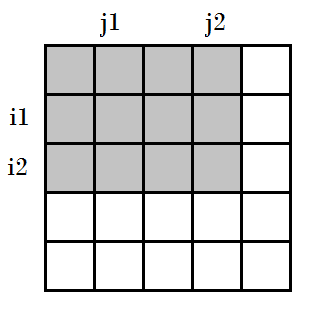
\includegraphics[scale=0.4]{Estructuras_de_datos/imagenes/img1}
			\caption{}%\label{fig:awesome_image1}
		\endminipage
		\minipage{0.25\textwidth}
			\centering
			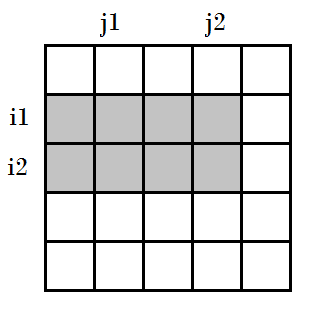
\includegraphics[scale=0.4]{Estructuras_de_datos/imagenes/img2}
			\caption{}
		\endminipage
		\minipage{0.25\textwidth}
			\centering
			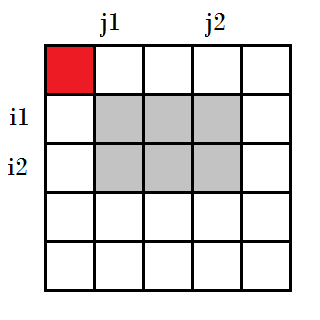
\includegraphics[scale=0.4]{Estructuras_de_datos/imagenes/img3}
			\caption{}%\label{fig:awesome_image1}
		\endminipage
		\minipage{0.25\textwidth}
			\centering
			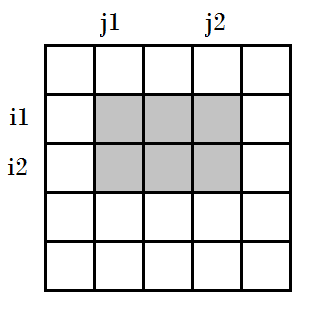
\includegraphics[scale=0.4]{Estructuras_de_datos/imagenes/img4}
			\caption{}
		\endminipage
	\end{figure}
	
	Para la solución en C++ la fila y columna cero de la tabla donde se guardara el pre-calculo se deberá llenar
	con el elemento neutro, el cero, luego se debe llenar el resto de la tabla siguiendo las formulas antes 
	establecidas, este ejemplo es para consultas indexando desde 1.
	\cppfile[26-36]{Estructuras_de_datos/codigos/tablas_aditivas.cpp}
	
	\subtitulo{Tablas aditivas en 3D}
	
	Las tablas aditivas se pueden generalizar para trabajar en n-dimensiones, mas sin embargo la dificultad de hacer 
	los pre-cálculos y las consultas aumenta bastante, pues crece considerablemente la cantidad de operaciones a
	realizar. En el caso 3D igualmente se debe tener cuidado con el principio de inclusión-exclusión, el 
	pre-calculo se realizaría de la siguiente manera: sea 
	$suma(i,j,k)$ = $\sum_{x=1}^{i} \sum_{y=1}^{j} \sum_{z=1}^{k} V_{x,y,z}$, entonces  
	$suma(i,j,k) = V_{i,j,k} + suma(i,j,k-1)+suma(i-1,j,k)+suma(i,j-1,k)-suma(i-1,j-1,k)-suma(i-1,j,k-1)
	-suma(i,j-1,k-1)+suma(i-1,j-1,k-1)$, y para las consultas: $\sum_{x=i1}^{i2} \sum_{y=j1}^{j2} \sum_{z=k1}^{k2}
	V_{x,y,z} = suma(i2,j2,k2)-suma(i2,j2,k1-1)-suma(i1-1,j2,k2)+suma(i1-1,j2,k1-1)-suma(i2,j1-1,k2)
	+suma(i2,j1-1,k1-1)+suma(i1-1,j1-1,k2)-suma(i1-1,j1-1,k1-1)$.
	
	Esta estructura de datos puede ser aplicada para otras operaciones que cumplan con las tres propiedades descritas
	anteriormente, la complejidad computacional de hacer el pre-calculo es lineal a la cantidad de
	elementos en la estructura, y las consultas se realizan en complejidad constante al realizar solamente operaciones
	directas sobre elementos en la tabla del pre-calculo.
	
	\section{Bibliografia}
	
	%https://en.wikipedia.org/wiki/Summed-area_table.\\ 
	http://trainingcamp.org.ar/anteriores/2017/clases.shtml.\\ 
	libro: competitive programming 3.\\ 

	%</Capitulo>
	
\end{document}



